\documentclass[tikz,border=8pt]{standalone}
% Shared look for every TikZ diagram. Load with \input{../../tools/tikz-style.tex}
\usepackage[T1]{fontenc}
\usepackage{lmodern}
\renewcommand{\sfdefault}{lmr}  % diagrams use the same serif as the text
\usetikzlibrary{arrows.meta, positioning, shapes.geometric, calc, fit, backgrounds}
\definecolor{cblue}{HTML}{4C78A8}
\definecolor{corange}{HTML}{F58518}
\definecolor{cgreen}{HTML}{54A24B}
\definecolor{cred}{HTML}{E45756}
\definecolor{cpurple}{HTML}{B279A2}
\definecolor{cgrey}{HTML}{6B6B6B}
\tikzset{
  every picture/.style={font=\sffamily, line width=1.2pt},
  box/.style={draw=#1, fill=#1!12, rounded corners=4pt, align=center, inner sep=7pt, minimum height=1.1cm},
  box/.default=cgrey,
  arrow/.style={-{Stealth[length=3mm]}, draw=cgrey, line width=1.4pt},
  title/.style={font=\sffamily\bfseries\Large},
  note/.style={font=\sffamily\small, text=cgrey, align=center},
}
\AtBeginDocument{\hyphenpenalty=10000 \exhyphenpenalty=10000}

\begin{document}
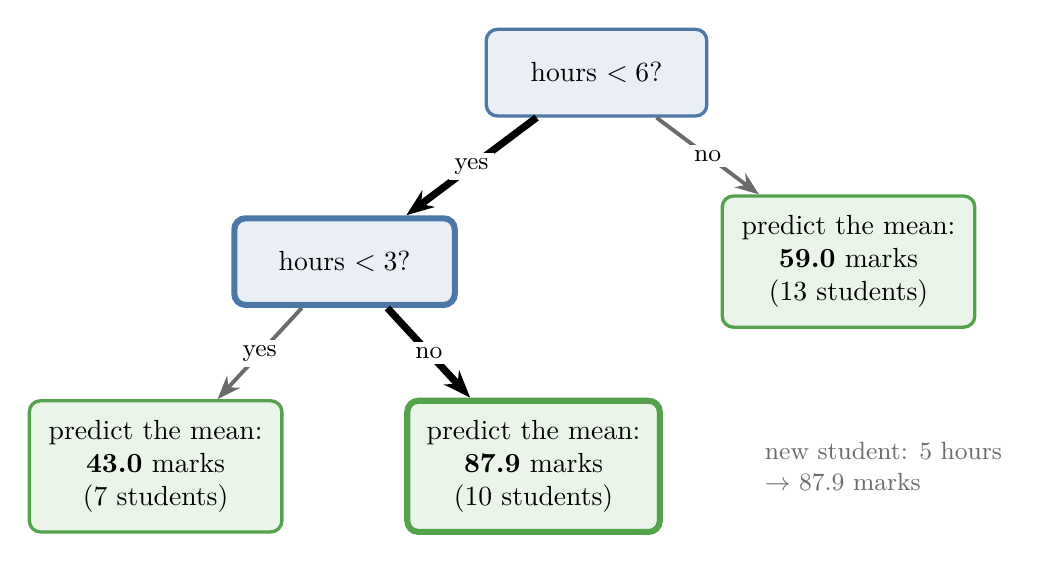
\begin{tikzpicture}[
  q/.style={box=cblue, minimum width=2.8cm},
  leaf/.style={box=cgreen, minimum width=3.2cm},
  lab/.style={font=\sffamily\small, fill=white, inner sep=2pt},
  path/.style={-{Stealth[length=3.5mm]}, draw=black, line width=2.6pt}]
  \node[q] (r) at (0,0) {hours $< 6$?};
  \node[q, line width=2.2pt] (s) at (-3.2,-2.4) {hours $< 3$?};
  \node[leaf] (c) at (3.2,-2.4) {predict the mean:\\\textbf{59.0} marks\\(13 students)};
  \node[leaf] (a) at (-5.6,-5.0) {predict the mean:\\\textbf{43.0} marks\\(7 students)};
  \node[leaf, line width=2.2pt] (b) at (-0.8,-5.0) {predict the mean:\\\textbf{87.9} marks\\(10 students)};
  \draw[path] (r) -- node[lab] {yes} (s);
  \draw[arrow] (r) -- node[lab] {no} (c);
  \draw[arrow] (s) -- node[lab] {yes} (a);
  \draw[path] (s) -- node[lab] {no} (b);
  \node[note, anchor=west, align=left] at (2.0,-5.0) {new student: 5 hours\\$\rightarrow$ 87.9 marks};
\end{tikzpicture}
\end{document}
